\chapter{Einleitung}
\label{chap:einleitung}

\section{Grundlagen}
\label{sec:Grundlagen}
Grundsätzlich ist das in dieser Arbeit behandelnde Thema für jede Person mit einer allgemeinen Informatikausbildung ohne weiteres zu verstehen. Es wird bei dieser Personengruppe, die Kenntnisse über grundsätzliche Architekturen innerhalb der IT vorausgesetzt. Zudem kann vorausgesetzt werden, dass jede Person dieser Gruppe, der englischen Sprache mächtig ist. Weiterhin sollen  einige Begrifflichkeiten geklärt werden, welche für die Arbeit notwendig sind:

\subsection{Time-to-Market (TTM}
\label{subsec:ttm}
Unter dem Begriff Time-to-Market wird die Zeit von der Produktentwicklung bis zur Auslieferung auf dem Markt verstanden.\footnote{Vergleich mit \cite{ttm:BusinessDictionary}}  In dieser Zeit müssen Kosten für die Erstellung/Entwicklung aufgebracht werden, es werden in dieser Zeit jedoch keine Umsätze erzeugt. Daher strebt jedes Unternehmen eine möglichst geringe Time-to-Market Zeit an. Insbesondere wenn es um Wettbewerb geht, muss diese Zeit kurz gehalten werden.

\subsection{Wertschöpfungskette}
\label{subsec:Wertschoepfungskette}
\begin{quotation}
\frqq Die Wertschöpfungskette stellt die zusammenhängenden Unternehmensaktivitäten des betrieblichen Gütererstellungsprozesses grafisch dar.\flqq \cite{gabler}
\end{quotation}

\begin{figure}[htb]
    \centering 
    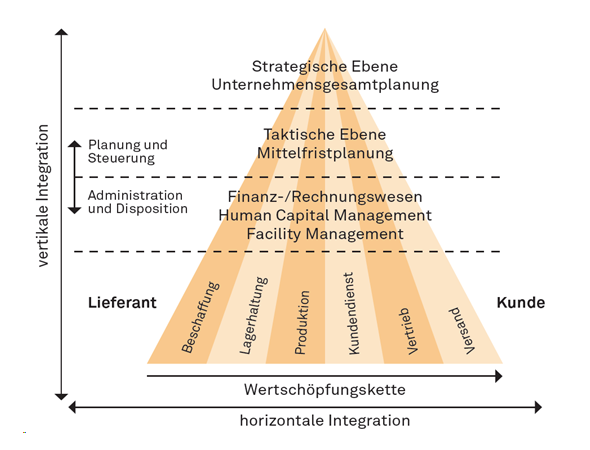
\includegraphics[width=\linewidth]{content/images/integrations-pyramide}\
    \quelle\url{http://www.referenzportal.ch/fuehrung/vom-erp-zum-integrierten-informationssystem/}
    \caption[Darstellung einer typischen Integrations-Pyramide]{Darstellung einer typischen Integrations-Pyramide\\}
    \label{fig:integrations-pyramide} 
\end{figure} 
Das Bild zeigt eine typische Integrations-Pyramide eines Unternehmens. In dieser Pyramide ist zum einen ersichtlich das für die Wertschöpfungskette die horizontale Integration wichtig ist, zum anderen jedoch auch, dass mehrere Abteilungen eines Unternehmens in einer Wertschöpfungskette durchlaufen werden müssen.
\\\\
Die Dauer zum durchlaufen der Wertschöpfungskette nennt man auch Time-to-Market. Wird die Kette daher in möglichst geringer Zeit durchlaufen, wird die Time-to-Market Zeitspanne verringert.

\section{Begriffsabgrenzung}
\label{sec:Begriffsabgrenzung}

\subsection*{SOA}
Sowohl SOA als auch Microservices zählen zu dem Paradigma der "`Service-orientierten Architekturen"'.

Die Abkürzung SOA wird hier sowohl für das Paradigma "`Service-orientierte Architektur"' verwendet, wie auch der speziellen Herangehensweise.

Um die beiden Thematiken in dieser Arbeit abzugrenzen wird der Begriff "`SOA"' für die Herangehensweise verwendet und die ausgeschriebene Variante zur Kennzeichnung des allgemeinen Paradigmas.

%\subsection*{Microservice}
%Der Begriff Microservice wird einerseits zum Beschreiben eines Architekturmodells genutzt, als auch zum beschreiben von eigenständigen Diensten (Services).

%Damit keine Verwechslung entsteht, wird in dieser Arbeit der Begriff "`Microservice"' verwendet, sofern das Architekturmodell gemeint ist und der Begriff "`Dienst"' oder "`Service"', wenn ein eigenständiger Dienst gemeint ist.

\section{Motivation}
\label{sec:motivation}
Die Anforderungen an Software werden zunehmend komplexer. Sie muss nicht nur funktionieren, sondern müssen zum Teil in kürzester Zeit erweitert oder geändert werden, was eine besondere Herausforderung dar stellt. Dabei spielen sowohl Funktionale, als auch nicht Funktionale Anforderungen eine wichtige Rolle. Je komplexer Software wird, desto schwieriger ist sie zu warten und zu pflegen. 

\begin{quotation}
\frqq Die Zeitspanne des Time-to-Market [(TTM)] kann [dabei] ein sehr bedeutsamer Faktor für den Erfolg des Unternehmens darstellen und ist daher nicht zu vernachlässigen. Kurze Entwicklungszeiträume bei der Time-to-Market garantieren dem Unternehmen nämlich einen Vorteil gegenüber der Konkurrenz. Hier geht es darum, dem Kunden so schnell wie möglich ein neues und innovatives Produkt anbieten zu können.
    
Um den Erfolg durch eine kurze Time-to-Market zu unterstützen und zu fördern, investieren Unternehmen in ihre Entwicklungsabteilungen. Diese können sich so nur auf ihre jeweiligen Bereiche konzentrieren. Durch eine leistungsfähige Entwicklungsabteilung kann so, in Kombination mit einem gut organisierten Projektplan und eindeutigen Zuständigkeiten, die Zeitspanne Time-to-Market so klein wie möglich gehalten werden. Gerade in Branchen, in denen Innovation eine übergeordnete Rolle spielt und der Produkt-Lebens-Zyklus generell eher kurz ausfällt, spielt eine kurze Time-to-Market eine außerordentlich wichtige Rolle.\flqq \cite{ttm}
\end{quotation}

Zusätzlich entstehen Kosten für die Planung und Entwicklung des Produktes. Bis zur Veröffentlichung des Produktes hat das Unternehmen Geld und Zeit investiert. Je länger die Zeitspanne des TTM ist, umso erfolgreicher muss das Produkt sein, bzw. der Preis groß genug sein, damit möglichst zeitnah der Break-even-Point, also die Schwelle, ab der die Produktionskosten wieder eingenommen worden sind und ein Gewinn entsteht, erreicht wird.

Zudem gibt es in einem Unternehmen nicht nur ein Software Produkt, sondern eine viel Zahl verschiedener Produkte für unterschiedliche Anwendungsfälle. Dabei kann es passieren, dass einige Anwendungen gleiche Funktionalitäten beinhalten. Müssen solche Funktionalitäten geändert werden, müssen dafür alle Anwendungen, welche diese Funktionen bereitstellen, geändert werden. Einfacher ist es daher, nur eine Anwendung zu haben, welches diese Funktionalität anbietet. Dadurch bedarf es nicht mehr die Anpassung von vielen Anwendungen, sondern nur noch von dieser einen.

\section{Ausgangssituation}
\label{sec:ausgangssituation}
Bei der Ausgangssituation handelt es sich um ein fiktives Szenario, welches an ein reales Problem
angelehnt ist.
\\\\
Das Unternehmen \textit{Auktionen GmbH}\ ist ein modernes und aktives Internet-Unternehmen, welches seit 1995 existiert. Wie der Name schon sagt, betreibt das Unternehmen eine Auktionsplattform im Internet. Diese wurde zunächst als monolithische Anwendung implementiert.
\\\\
Mit zunehmenden Nutzerzahlen und damit täglichen Benutzungen, stellte das Unternehmen fest, dass es zunehmend schwieriger wurde, auf das Verhalten der Nutzer in angemessener Zeit zu reagieren. Da die zentrale Anwendung ein monolithisches System war, war es zudem schwierig diese zu deployen.
\\\\
Musste eine neue Version herausgebracht werden, so bedeutet dies entweder die gesamte Infrastruktur für Wartungszwecke offline zu nehmen und die Anwendung neu zu deployen oder Server im Parallel betrieb laufen zu lassen und jeden neuen Besucher auf die neue Version zu leiten. Die letzte Methode bietet jedoch einige Schwierigkeiten, denn es könnten Änderungen eingebaut worden sein, welche im Konflikt mit der alten Version stehen. Dann muss in jedem Fall die erste Variante gewählt werden und die gesamte Infrastruktur offline genommen werden.
\\\\
Beide Varianten der Änderungen sind jedoch zeitaufwendig und schwierig, denn nicht nur das deployen könnte Probleme bereiten, sondern auch die darauf folgende Ausführung des Programms. Ändert man Code in monolithischen Applikationen kann das auch Auswirkungen auf bestehende Teile des Codes haben, welche vorher, ohne Probleme, funktioniert haben. Werden Tests vernachlässigt oder wird nicht ausreichend getestet, kann es leicht passieren, dass sich Fehler einschleichen, wodurch dann eine Version in betrieb genommen wird, welche Fehler enthält. Darauf folgend müssten diese wieder behoben werden und die Anwendung erneut deployed werden.
\\\\
Im Falle einer monolithischen Architektur bedeutet das viele Änderungen und neue Features. Oft passiert es daher, dass Code Stücke zurückbleiben, welche nicht mehr benötigt werden. Irgendwann ist die Applikation daher so groß, dass sie nicht mehr Wartbar ist und neue Features nur noch schwer zu implementieren sind. Entstehen Fehler in solch einer Anwendung ist es um so schwerer diese zu finden und zu beheben.
\\\\
Aus diesem Grund hat die \textit{Auktionen GmbH} sich entschlossen, die monolithische Strukturen nicht weiter zu entwickeln, sondern auf ein Service-orientierte Architektur umzustellen.

\section{Vorgehen und Kapitel}
\label{sec:vorgehen}
Zunächst werden die Probleme bei der Verwendung von monolithischen Architekturen, unter dem Aspekt der Softwareentwicklung und Wartung analysiert. Darauf aufbauend soll die Grundlegende Problematik herausgearbeitet werden. Anschließend werden die Grundlagen zur Verwendung von Service orientierten Architekturen und deren Vorteile, aufbauend auf die zuvor erläuterte Problematik, erklärt. In den Grundlagen werden außerdem Werkzeuge erklärt, mit deren Hilfe solche Architekturen realisiert werden können und die Wartung vereinfachen.
\\
Darauf folgend wird das Architekturparadigma "'Microservice"' unter der Verwendung von den erläuterten Werkzeugen erklärt und der Begriff Continuous Delivery eingeführt. Anschließend wird, unter Verwendung des angeeigneten Wissens aus dem Kapitel "'Microservice"', auf das Architekturparadigma "'Service-orientierte Architektur (SOA)"' eingegangen.
\\
Abschließend werden die gewonnen Kenntnisse zusammengetragen und Ausgewertet. Dabei sollen beide Architekturparadigmen verglichen und bewertet werden. Zuletzt wird das Thema noch einmal zusammengefasst und ein Ausblick auf kommende Projekte bzw. die Bachelorarbeit gegeben.